% Created by tikzDevice version 0.12.6 on 2026-02-05 15:17:19
% !TEX encoding = UTF-8 Unicode
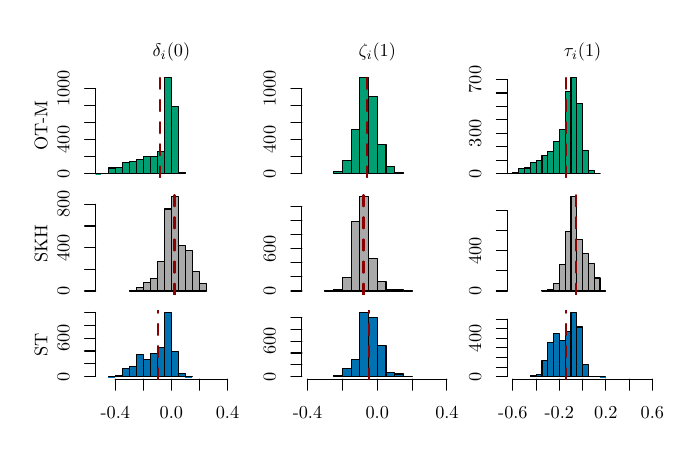
\begin{tikzpicture}[x=1pt,y=1pt]
\definecolor{fillColor}{RGB}{255,255,255}
\path[use as bounding box,fill=fillColor,fill opacity=0.00] (0,0) rectangle (230.90,143.67);
\begin{scope}
\path[clip] ( 24.55, 89.54) rectangle ( 79.30,127.04);
\definecolor{drawColor}{RGB}{0,0,0}
\definecolor{fillColor}{RGB}{0,158,115}

\path[draw=drawColor,line width= 0.4pt,line join=round,line cap=round,fill=fillColor] ( 24.05, 90.93) rectangle ( 26.58, 90.96);

\path[draw=drawColor,line width= 0.4pt,line join=round,line cap=round,fill=fillColor] ( 26.58, 90.93) rectangle ( 29.11, 91.09);

\path[draw=drawColor,line width= 0.4pt,line join=round,line cap=round,fill=fillColor] ( 29.11, 90.93) rectangle ( 31.65, 92.96);

\path[draw=drawColor,line width= 0.4pt,line join=round,line cap=round,fill=fillColor] ( 31.65, 90.93) rectangle ( 34.18, 93.30);

\path[draw=drawColor,line width= 0.4pt,line join=round,line cap=round,fill=fillColor] ( 34.18, 90.93) rectangle ( 36.72, 94.90);

\path[draw=drawColor,line width= 0.4pt,line join=round,line cap=round,fill=fillColor] ( 36.72, 90.93) rectangle ( 39.25, 95.24);

\path[draw=drawColor,line width= 0.4pt,line join=round,line cap=round,fill=fillColor] ( 39.25, 90.93) rectangle ( 41.79, 96.13);

\path[draw=drawColor,line width= 0.4pt,line join=round,line cap=round,fill=fillColor] ( 41.79, 90.93) rectangle ( 44.32, 97.06);

\path[draw=drawColor,line width= 0.4pt,line join=round,line cap=round,fill=fillColor] ( 44.32, 90.93) rectangle ( 46.86, 97.27);

\path[draw=drawColor,line width= 0.4pt,line join=round,line cap=round,fill=fillColor] ( 46.86, 90.93) rectangle ( 49.39, 98.84);

\path[draw=drawColor,line width= 0.4pt,line join=round,line cap=round,fill=fillColor] ( 49.39, 90.93) rectangle ( 51.92,125.65);

\path[draw=drawColor,line width= 0.4pt,line join=round,line cap=round,fill=fillColor] ( 51.92, 90.93) rectangle ( 54.46,115.12);

\path[draw=drawColor,line width= 0.4pt,line join=round,line cap=round,fill=fillColor] ( 54.46, 90.93) rectangle ( 56.99, 91.30);
\end{scope}
\begin{scope}
\path[clip] (  0.00,  0.00) rectangle (230.90,143.67);
\definecolor{drawColor}{RGB}{0,0,0}

\path[draw=drawColor,line width= 0.4pt,line join=round,line cap=round] ( 24.55, 90.93) -- ( 24.55,121.71);

\path[draw=drawColor,line width= 0.4pt,line join=round,line cap=round] ( 24.55, 90.93) -- ( 20.59, 90.93);

\path[draw=drawColor,line width= 0.4pt,line join=round,line cap=round] ( 24.55, 97.09) -- ( 20.59, 97.09);

\path[draw=drawColor,line width= 0.4pt,line join=round,line cap=round] ( 24.55,103.24) -- ( 20.59,103.24);

\path[draw=drawColor,line width= 0.4pt,line join=round,line cap=round] ( 24.55,109.40) -- ( 20.59,109.40);

\path[draw=drawColor,line width= 0.4pt,line join=round,line cap=round] ( 24.55,115.56) -- ( 20.59,115.56);

\path[draw=drawColor,line width= 0.4pt,line join=round,line cap=round] ( 24.55,121.71) -- ( 20.59,121.71);

\node[text=drawColor,rotate= 90.00,anchor=base,inner sep=0pt, outer sep=0pt, scale=  0.66] at ( 15.05, 90.93) {0};

\node[text=drawColor,rotate= 90.00,anchor=base,inner sep=0pt, outer sep=0pt, scale=  0.66] at ( 15.05,103.24) {400};

\node[text=drawColor,rotate= 90.00,anchor=base,inner sep=0pt, outer sep=0pt, scale=  0.66] at ( 15.05,121.71) {1000};
\end{scope}
\begin{scope}
\path[clip] (  0.00, 84.79) rectangle ( 82.47,143.67);
\definecolor{drawColor}{RGB}{0,0,0}

\node[text=drawColor,anchor=base,inner sep=0pt, outer sep=0pt, scale=  0.66] at ( 51.92,133.08) {\bfseries $\delta_i(0)$};

\node[text=drawColor,rotate= 90.00,anchor=base,inner sep=0pt, outer sep=0pt, scale=  0.66] at (  7.13,108.29) {OT-M};
\end{scope}
\begin{scope}
\path[clip] ( 24.55, 89.54) rectangle ( 79.30,127.04);
\definecolor{drawColor}{RGB}{139,0,0}

\path[draw=drawColor,line width= 0.8pt,dash pattern=on 4pt off 4pt ,line join=round,line cap=round] ( 47.70, 89.54) -- ( 47.70,127.04);
\end{scope}
\begin{scope}
\path[clip] ( 99.10, 89.54) rectangle (153.52,127.04);
\definecolor{drawColor}{RGB}{0,0,0}
\definecolor{fillColor}{RGB}{0,158,115}

\path[draw=drawColor,line width= 0.4pt,line join=round,line cap=round,fill=fillColor] (110.56, 90.93) rectangle (113.71, 91.58);

\path[draw=drawColor,line width= 0.4pt,line join=round,line cap=round,fill=fillColor] (113.71, 90.93) rectangle (116.86, 95.83);

\path[draw=drawColor,line width= 0.4pt,line join=round,line cap=round,fill=fillColor] (116.86, 90.93) rectangle (120.01,107.01);

\path[draw=drawColor,line width= 0.4pt,line join=round,line cap=round,fill=fillColor] (120.01, 90.93) rectangle (123.16,125.65);

\path[draw=drawColor,line width= 0.4pt,line join=round,line cap=round,fill=fillColor] (123.16, 90.93) rectangle (126.31,118.94);

\path[draw=drawColor,line width= 0.4pt,line join=round,line cap=round,fill=fillColor] (126.31, 90.93) rectangle (129.46,101.41);

\path[draw=drawColor,line width= 0.4pt,line join=round,line cap=round,fill=fillColor] (129.46, 90.93) rectangle (132.61, 93.43);

\path[draw=drawColor,line width= 0.4pt,line join=round,line cap=round,fill=fillColor] (132.61, 90.93) rectangle (135.75, 91.42);
\end{scope}
\begin{scope}
\path[clip] (  0.00,  0.00) rectangle (230.90,143.67);
\definecolor{drawColor}{RGB}{0,0,0}

\path[draw=drawColor,line width= 0.4pt,line join=round,line cap=round] ( 99.10, 90.93) -- ( 99.10,121.74);

\path[draw=drawColor,line width= 0.4pt,line join=round,line cap=round] ( 99.10, 90.93) -- ( 95.14, 90.93);

\path[draw=drawColor,line width= 0.4pt,line join=round,line cap=round] ( 99.10, 97.09) -- ( 95.14, 97.09);

\path[draw=drawColor,line width= 0.4pt,line join=round,line cap=round] ( 99.10,103.25) -- ( 95.14,103.25);

\path[draw=drawColor,line width= 0.4pt,line join=round,line cap=round] ( 99.10,109.42) -- ( 95.14,109.42);

\path[draw=drawColor,line width= 0.4pt,line join=round,line cap=round] ( 99.10,115.58) -- ( 95.14,115.58);

\path[draw=drawColor,line width= 0.4pt,line join=round,line cap=round] ( 99.10,121.74) -- ( 95.14,121.74);

\node[text=drawColor,rotate= 90.00,anchor=base,inner sep=0pt, outer sep=0pt, scale=  0.66] at ( 89.59, 90.93) {0};

\node[text=drawColor,rotate= 90.00,anchor=base,inner sep=0pt, outer sep=0pt, scale=  0.66] at ( 89.59,103.25) {400};

\node[text=drawColor,rotate= 90.00,anchor=base,inner sep=0pt, outer sep=0pt, scale=  0.66] at ( 89.59,121.74) {1000};
\end{scope}
\begin{scope}
\path[clip] ( 82.47, 84.79) rectangle (156.68,143.67);
\definecolor{drawColor}{RGB}{0,0,0}

\node[text=drawColor,anchor=base,inner sep=0pt, outer sep=0pt, scale=  0.66] at (126.31,133.08) {\bfseries $\zeta_i(1)$};
\end{scope}
\begin{scope}
\path[clip] ( 99.10, 89.54) rectangle (153.52,127.04);
\definecolor{drawColor}{RGB}{139,0,0}

\path[draw=drawColor,line width= 0.8pt,dash pattern=on 4pt off 4pt ,line join=round,line cap=round] (122.57, 89.54) -- (122.57,127.04);
\end{scope}
\begin{scope}
\path[clip] (173.32, 89.54) rectangle (227.73,127.04);
\definecolor{drawColor}{RGB}{0,0,0}
\definecolor{fillColor}{RGB}{0,158,115}

\path[draw=drawColor,line width= 0.4pt,line join=round,line cap=round,fill=fillColor] (173.23, 90.93) rectangle (175.33, 90.98);

\path[draw=drawColor,line width= 0.4pt,line join=round,line cap=round,fill=fillColor] (175.33, 90.93) rectangle (177.43, 91.27);

\path[draw=drawColor,line width= 0.4pt,line join=round,line cap=round,fill=fillColor] (177.43, 90.93) rectangle (179.53, 92.63);

\path[draw=drawColor,line width= 0.4pt,line join=round,line cap=round,fill=fillColor] (179.53, 90.93) rectangle (181.63, 92.97);

\path[draw=drawColor,line width= 0.4pt,line join=round,line cap=round,fill=fillColor] (181.63, 90.93) rectangle (183.73, 95.11);

\path[draw=drawColor,line width= 0.4pt,line join=round,line cap=round,fill=fillColor] (183.73, 90.93) rectangle (185.83, 95.74);

\path[draw=drawColor,line width= 0.4pt,line join=round,line cap=round,fill=fillColor] (185.83, 90.93) rectangle (187.93, 97.34);

\path[draw=drawColor,line width= 0.4pt,line join=round,line cap=round,fill=fillColor] (187.93, 90.93) rectangle (190.03, 99.04);

\path[draw=drawColor,line width= 0.4pt,line join=round,line cap=round,fill=fillColor] (190.03, 90.93) rectangle (192.13,102.44);

\path[draw=drawColor,line width= 0.4pt,line join=round,line cap=round,fill=fillColor] (192.13, 90.93) rectangle (194.23,106.81);

\path[draw=drawColor,line width= 0.4pt,line join=round,line cap=round,fill=fillColor] (194.23, 90.93) rectangle (196.33,120.50);

\path[draw=drawColor,line width= 0.4pt,line join=round,line cap=round,fill=fillColor] (196.33, 90.93) rectangle (198.43,125.65);

\path[draw=drawColor,line width= 0.4pt,line join=round,line cap=round,fill=fillColor] (198.43, 90.93) rectangle (200.53,116.38);

\path[draw=drawColor,line width= 0.4pt,line join=round,line cap=round,fill=fillColor] (200.53, 90.93) rectangle (202.62, 99.14);

\path[draw=drawColor,line width= 0.4pt,line join=round,line cap=round,fill=fillColor] (202.62, 90.93) rectangle (204.72, 91.95);

\path[draw=drawColor,line width= 0.4pt,line join=round,line cap=round,fill=fillColor] (204.72, 90.93) rectangle (206.82, 91.13);
\end{scope}
\begin{scope}
\path[clip] (  0.00,  0.00) rectangle (230.90,143.67);
\definecolor{drawColor}{RGB}{0,0,0}

\path[draw=drawColor,line width= 0.4pt,line join=round,line cap=round] (173.32, 90.93) -- (173.32,124.92);

\path[draw=drawColor,line width= 0.4pt,line join=round,line cap=round] (173.32, 90.93) -- (169.36, 90.93);

\path[draw=drawColor,line width= 0.4pt,line join=round,line cap=round] (173.32, 95.79) -- (169.36, 95.79);

\path[draw=drawColor,line width= 0.4pt,line join=round,line cap=round] (173.32,100.64) -- (169.36,100.64);

\path[draw=drawColor,line width= 0.4pt,line join=round,line cap=round] (173.32,105.50) -- (169.36,105.50);

\path[draw=drawColor,line width= 0.4pt,line join=round,line cap=round] (173.32,110.36) -- (169.36,110.36);

\path[draw=drawColor,line width= 0.4pt,line join=round,line cap=round] (173.32,115.21) -- (169.36,115.21);

\path[draw=drawColor,line width= 0.4pt,line join=round,line cap=round] (173.32,120.07) -- (169.36,120.07);

\path[draw=drawColor,line width= 0.4pt,line join=round,line cap=round] (173.32,124.92) -- (169.36,124.92);

\node[text=drawColor,rotate= 90.00,anchor=base,inner sep=0pt, outer sep=0pt, scale=  0.66] at (163.81, 90.93) {0};

\node[text=drawColor,rotate= 90.00,anchor=base,inner sep=0pt, outer sep=0pt, scale=  0.66] at (163.81,105.50) {300};

\node[text=drawColor,rotate= 90.00,anchor=base,inner sep=0pt, outer sep=0pt, scale=  0.66] at (163.81,124.92) {700};
\end{scope}
\begin{scope}
\path[clip] (156.68, 84.79) rectangle (230.90,143.67);
\definecolor{drawColor}{RGB}{0,0,0}

\node[text=drawColor,anchor=base,inner sep=0pt, outer sep=0pt, scale=  0.66] at (200.53,133.08) {\bfseries $\tau_i(1)$};
\end{scope}
\begin{scope}
\path[clip] (173.32, 89.54) rectangle (227.73,127.04);
\definecolor{drawColor}{RGB}{139,0,0}

\path[draw=drawColor,line width= 0.8pt,dash pattern=on 4pt off 4pt ,line join=round,line cap=round] (194.54, 89.54) -- (194.54,127.04);
\end{scope}
\begin{scope}
\path[clip] ( 24.55, 47.15) rectangle ( 79.30, 84.00);
\definecolor{drawColor}{RGB}{0,0,0}
\definecolor{fillColor}{RGB}{169,169,169}

\path[draw=drawColor,line width= 0.4pt,line join=round,line cap=round,fill=fillColor] ( 36.72, 48.51) rectangle ( 39.25, 48.75);

\path[draw=drawColor,line width= 0.4pt,line join=round,line cap=round,fill=fillColor] ( 39.25, 48.51) rectangle ( 41.79, 49.92);

\path[draw=drawColor,line width= 0.4pt,line join=round,line cap=round,fill=fillColor] ( 41.79, 48.51) rectangle ( 44.32, 51.49);

\path[draw=drawColor,line width= 0.4pt,line join=round,line cap=round,fill=fillColor] ( 44.32, 48.51) rectangle ( 46.86, 53.13);

\path[draw=drawColor,line width= 0.4pt,line join=round,line cap=round,fill=fillColor] ( 46.86, 48.51) rectangle ( 49.39, 59.17);

\path[draw=drawColor,line width= 0.4pt,line join=round,line cap=round,fill=fillColor] ( 49.39, 48.51) rectangle ( 51.92, 78.13);

\path[draw=drawColor,line width= 0.4pt,line join=round,line cap=round,fill=fillColor] ( 51.92, 48.51) rectangle ( 54.46, 82.63);

\path[draw=drawColor,line width= 0.4pt,line join=round,line cap=round,fill=fillColor] ( 54.46, 48.51) rectangle ( 56.99, 65.00);

\path[draw=drawColor,line width= 0.4pt,line join=round,line cap=round,fill=fillColor] ( 56.99, 48.51) rectangle ( 59.53, 63.16);

\path[draw=drawColor,line width= 0.4pt,line join=round,line cap=round,fill=fillColor] ( 59.53, 48.51) rectangle ( 62.06, 55.45);

\path[draw=drawColor,line width= 0.4pt,line join=round,line cap=round,fill=fillColor] ( 62.06, 48.51) rectangle ( 64.60, 51.18);
\end{scope}
\begin{scope}
\path[clip] (  0.00,  0.00) rectangle (230.90,143.67);
\definecolor{drawColor}{RGB}{0,0,0}

\path[draw=drawColor,line width= 0.4pt,line join=round,line cap=round] ( 24.55, 48.51) -- ( 24.55, 79.85);

\path[draw=drawColor,line width= 0.4pt,line join=round,line cap=round] ( 24.55, 48.51) -- ( 20.59, 48.51);

\path[draw=drawColor,line width= 0.4pt,line join=round,line cap=round] ( 24.55, 56.35) -- ( 20.59, 56.35);

\path[draw=drawColor,line width= 0.4pt,line join=round,line cap=round] ( 24.55, 64.18) -- ( 20.59, 64.18);

\path[draw=drawColor,line width= 0.4pt,line join=round,line cap=round] ( 24.55, 72.02) -- ( 20.59, 72.02);

\path[draw=drawColor,line width= 0.4pt,line join=round,line cap=round] ( 24.55, 79.85) -- ( 20.59, 79.85);

\node[text=drawColor,rotate= 90.00,anchor=base,inner sep=0pt, outer sep=0pt, scale=  0.66] at ( 15.05, 48.51) {0};

\node[text=drawColor,rotate= 90.00,anchor=base,inner sep=0pt, outer sep=0pt, scale=  0.66] at ( 15.05, 64.18) {400};

\node[text=drawColor,rotate= 90.00,anchor=base,inner sep=0pt, outer sep=0pt, scale=  0.66] at ( 15.05, 79.85) {800};
\end{scope}
\begin{scope}
\path[clip] (  0.00, 42.40) rectangle ( 82.47, 84.79);
\definecolor{drawColor}{RGB}{0,0,0}

\node[text=drawColor,rotate= 90.00,anchor=base,inner sep=0pt, outer sep=0pt, scale=  0.66] at (  7.13, 65.57) {SKH};
\end{scope}
\begin{scope}
\path[clip] ( 24.55, 47.15) rectangle ( 79.30, 84.00);
\definecolor{drawColor}{RGB}{139,0,0}

\path[draw=drawColor,line width= 0.8pt,dash pattern=on 4pt off 4pt ,line join=round,line cap=round] ( 53.04, 47.15) -- ( 53.04, 84.00);
\end{scope}
\begin{scope}
\path[clip] ( 99.10, 47.15) rectangle (153.52, 84.00);
\definecolor{drawColor}{RGB}{0,0,0}
\definecolor{fillColor}{RGB}{169,169,169}

\path[draw=drawColor,line width= 0.4pt,line join=round,line cap=round,fill=fillColor] (107.41, 48.51) rectangle (110.56, 48.56);

\path[draw=drawColor,line width= 0.4pt,line join=round,line cap=round,fill=fillColor] (110.56, 48.51) rectangle (113.71, 49.17);

\path[draw=drawColor,line width= 0.4pt,line join=round,line cap=round,fill=fillColor] (113.71, 48.51) rectangle (116.86, 53.50);

\path[draw=drawColor,line width= 0.4pt,line join=round,line cap=round,fill=fillColor] (116.86, 48.51) rectangle (120.01, 73.47);

\path[draw=drawColor,line width= 0.4pt,line join=round,line cap=round,fill=fillColor] (120.01, 48.51) rectangle (123.16, 82.63);

\path[draw=drawColor,line width= 0.4pt,line join=round,line cap=round,fill=fillColor] (123.16, 48.51) rectangle (126.31, 60.10);

\path[draw=drawColor,line width= 0.4pt,line join=round,line cap=round,fill=fillColor] (126.31, 48.51) rectangle (129.46, 51.98);

\path[draw=drawColor,line width= 0.4pt,line join=round,line cap=round,fill=fillColor] (129.46, 48.51) rectangle (132.61, 49.15);

\path[draw=drawColor,line width= 0.4pt,line join=round,line cap=round,fill=fillColor] (132.61, 48.51) rectangle (135.75, 48.87);

\path[draw=drawColor,line width= 0.4pt,line join=round,line cap=round,fill=fillColor] (135.75, 48.51) rectangle (138.90, 48.54);
\end{scope}
\begin{scope}
\path[clip] (  0.00,  0.00) rectangle (230.90,143.67);
\definecolor{drawColor}{RGB}{0,0,0}

\path[draw=drawColor,line width= 0.4pt,line join=round,line cap=round] ( 99.10, 48.51) -- ( 99.10, 79.07);

\path[draw=drawColor,line width= 0.4pt,line join=round,line cap=round] ( 99.10, 48.51) -- ( 95.14, 48.51);

\path[draw=drawColor,line width= 0.4pt,line join=round,line cap=round] ( 99.10, 53.60) -- ( 95.14, 53.60);

\path[draw=drawColor,line width= 0.4pt,line join=round,line cap=round] ( 99.10, 58.70) -- ( 95.14, 58.70);

\path[draw=drawColor,line width= 0.4pt,line join=round,line cap=round] ( 99.10, 63.79) -- ( 95.14, 63.79);

\path[draw=drawColor,line width= 0.4pt,line join=round,line cap=round] ( 99.10, 68.88) -- ( 95.14, 68.88);

\path[draw=drawColor,line width= 0.4pt,line join=round,line cap=round] ( 99.10, 73.98) -- ( 95.14, 73.98);

\path[draw=drawColor,line width= 0.4pt,line join=round,line cap=round] ( 99.10, 79.07) -- ( 95.14, 79.07);

\node[text=drawColor,rotate= 90.00,anchor=base,inner sep=0pt, outer sep=0pt, scale=  0.66] at ( 89.59, 48.51) {0};

\node[text=drawColor,rotate= 90.00,anchor=base,inner sep=0pt, outer sep=0pt, scale=  0.66] at ( 89.59, 63.79) {600};
\end{scope}
\begin{scope}
\path[clip] ( 99.10, 47.15) rectangle (153.52, 84.00);
\definecolor{drawColor}{RGB}{139,0,0}

\path[draw=drawColor,line width= 0.8pt,dash pattern=on 4pt off 4pt ,line join=round,line cap=round] (121.36, 47.15) -- (121.36, 84.00);
\end{scope}
\begin{scope}
\path[clip] (173.32, 47.15) rectangle (227.73, 84.00);
\definecolor{drawColor}{RGB}{0,0,0}
\definecolor{fillColor}{RGB}{169,169,169}

\path[draw=drawColor,line width= 0.4pt,line join=round,line cap=round,fill=fillColor] (185.83, 48.51) rectangle (187.93, 48.55);

\path[draw=drawColor,line width= 0.4pt,line join=round,line cap=round,fill=fillColor] (187.93, 48.51) rectangle (190.03, 49.20);

\path[draw=drawColor,line width= 0.4pt,line join=round,line cap=round,fill=fillColor] (190.03, 48.51) rectangle (192.13, 51.23);

\path[draw=drawColor,line width= 0.4pt,line join=round,line cap=round,fill=fillColor] (192.13, 48.51) rectangle (194.23, 58.06);

\path[draw=drawColor,line width= 0.4pt,line join=round,line cap=round,fill=fillColor] (194.23, 48.51) rectangle (196.33, 69.89);

\path[draw=drawColor,line width= 0.4pt,line join=round,line cap=round,fill=fillColor] (196.33, 48.51) rectangle (198.43, 82.63);

\path[draw=drawColor,line width= 0.4pt,line join=round,line cap=round,fill=fillColor] (198.43, 48.51) rectangle (200.53, 67.02);

\path[draw=drawColor,line width= 0.4pt,line join=round,line cap=round,fill=fillColor] (200.53, 48.51) rectangle (202.62, 62.12);

\path[draw=drawColor,line width= 0.4pt,line join=round,line cap=round,fill=fillColor] (202.62, 48.51) rectangle (204.72, 58.39);

\path[draw=drawColor,line width= 0.4pt,line join=round,line cap=round,fill=fillColor] (204.72, 48.51) rectangle (206.82, 53.23);

\path[draw=drawColor,line width= 0.4pt,line join=round,line cap=round,fill=fillColor] (206.82, 48.51) rectangle (208.92, 48.55);
\end{scope}
\begin{scope}
\path[clip] (  0.00,  0.00) rectangle (230.90,143.67);
\definecolor{drawColor}{RGB}{0,0,0}

\path[draw=drawColor,line width= 0.4pt,line join=round,line cap=round] (173.32, 48.51) -- (173.32, 77.55);

\path[draw=drawColor,line width= 0.4pt,line join=round,line cap=round] (173.32, 48.51) -- (169.36, 48.51);

\path[draw=drawColor,line width= 0.4pt,line join=round,line cap=round] (173.32, 55.77) -- (169.36, 55.77);

\path[draw=drawColor,line width= 0.4pt,line join=round,line cap=round] (173.32, 63.03) -- (169.36, 63.03);

\path[draw=drawColor,line width= 0.4pt,line join=round,line cap=round] (173.32, 70.29) -- (169.36, 70.29);

\path[draw=drawColor,line width= 0.4pt,line join=round,line cap=round] (173.32, 77.55) -- (169.36, 77.55);

\node[text=drawColor,rotate= 90.00,anchor=base,inner sep=0pt, outer sep=0pt, scale=  0.66] at (163.81, 48.51) {0};

\node[text=drawColor,rotate= 90.00,anchor=base,inner sep=0pt, outer sep=0pt, scale=  0.66] at (163.81, 63.03) {400};
\end{scope}
\begin{scope}
\path[clip] (173.32, 47.15) rectangle (227.73, 84.00);
\definecolor{drawColor}{RGB}{139,0,0}

\path[draw=drawColor,line width= 0.8pt,dash pattern=on 4pt off 4pt ,line join=round,line cap=round] (198.15, 47.15) -- (198.15, 84.00);
\end{scope}
\begin{scope}
\path[clip] ( 24.55, 16.63) rectangle ( 79.30, 41.60);
\definecolor{drawColor}{RGB}{0,0,0}
\definecolor{fillColor}{RGB}{0,114,178}

\path[draw=drawColor,line width= 0.4pt,line join=round,line cap=round,fill=fillColor] ( 29.11, 17.56) rectangle ( 31.65, 17.58);

\path[draw=drawColor,line width= 0.4pt,line join=round,line cap=round,fill=fillColor] ( 31.65, 17.56) rectangle ( 34.18, 17.93);

\path[draw=drawColor,line width= 0.4pt,line join=round,line cap=round,fill=fillColor] ( 34.18, 17.56) rectangle ( 36.72, 20.53);

\path[draw=drawColor,line width= 0.4pt,line join=round,line cap=round,fill=fillColor] ( 36.72, 17.56) rectangle ( 39.25, 21.39);

\path[draw=drawColor,line width= 0.4pt,line join=round,line cap=round,fill=fillColor] ( 39.25, 17.56) rectangle ( 41.79, 25.52);

\path[draw=drawColor,line width= 0.4pt,line join=round,line cap=round,fill=fillColor] ( 41.79, 17.56) rectangle ( 44.32, 23.76);

\path[draw=drawColor,line width= 0.4pt,line join=round,line cap=round,fill=fillColor] ( 44.32, 17.56) rectangle ( 46.86, 26.08);

\path[draw=drawColor,line width= 0.4pt,line join=round,line cap=round,fill=fillColor] ( 46.86, 17.56) rectangle ( 49.39, 27.98);

\path[draw=drawColor,line width= 0.4pt,line join=round,line cap=round,fill=fillColor] ( 49.39, 17.56) rectangle ( 51.92, 40.68);

\path[draw=drawColor,line width= 0.4pt,line join=round,line cap=round,fill=fillColor] ( 51.92, 17.56) rectangle ( 54.46, 26.63);

\path[draw=drawColor,line width= 0.4pt,line join=round,line cap=round,fill=fillColor] ( 54.46, 17.56) rectangle ( 56.99, 18.74);

\path[draw=drawColor,line width= 0.4pt,line join=round,line cap=round,fill=fillColor] ( 56.99, 17.56) rectangle ( 59.53, 17.58);
\end{scope}
\begin{scope}
\path[clip] (  0.00,  0.00) rectangle (230.90,143.67);
\definecolor{drawColor}{RGB}{0,0,0}

\path[draw=drawColor,line width= 0.4pt,line join=round,line cap=round] ( 31.65, 16.63) -- ( 72.20, 16.63);

\path[draw=drawColor,line width= 0.4pt,line join=round,line cap=round] ( 31.65, 16.63) -- ( 31.65, 12.67);

\path[draw=drawColor,line width= 0.4pt,line join=round,line cap=round] ( 41.79, 16.63) -- ( 41.79, 12.67);

\path[draw=drawColor,line width= 0.4pt,line join=round,line cap=round] ( 51.92, 16.63) -- ( 51.92, 12.67);

\path[draw=drawColor,line width= 0.4pt,line join=round,line cap=round] ( 62.06, 16.63) -- ( 62.06, 12.67);

\path[draw=drawColor,line width= 0.4pt,line join=round,line cap=round] ( 72.20, 16.63) -- ( 72.20, 12.67);

\node[text=drawColor,anchor=base,inner sep=0pt, outer sep=0pt, scale=  0.66] at ( 31.65,  2.38) {-0.4};

\node[text=drawColor,anchor=base,inner sep=0pt, outer sep=0pt, scale=  0.66] at ( 51.92,  2.38) {0.0};

\node[text=drawColor,anchor=base,inner sep=0pt, outer sep=0pt, scale=  0.66] at ( 72.20,  2.38) {0.4};

\path[draw=drawColor,line width= 0.4pt,line join=round,line cap=round] ( 24.55, 17.56) -- ( 24.55, 40.77);

\path[draw=drawColor,line width= 0.4pt,line join=round,line cap=round] ( 24.55, 17.56) -- ( 20.59, 17.56);

\path[draw=drawColor,line width= 0.4pt,line join=round,line cap=round] ( 24.55, 22.20) -- ( 20.59, 22.20);

\path[draw=drawColor,line width= 0.4pt,line join=round,line cap=round] ( 24.55, 26.84) -- ( 20.59, 26.84);

\path[draw=drawColor,line width= 0.4pt,line join=round,line cap=round] ( 24.55, 31.49) -- ( 20.59, 31.49);

\path[draw=drawColor,line width= 0.4pt,line join=round,line cap=round] ( 24.55, 36.13) -- ( 20.59, 36.13);

\path[draw=drawColor,line width= 0.4pt,line join=round,line cap=round] ( 24.55, 40.77) -- ( 20.59, 40.77);

\node[text=drawColor,rotate= 90.00,anchor=base,inner sep=0pt, outer sep=0pt, scale=  0.66] at ( 15.05, 17.56) {0};

\node[text=drawColor,rotate= 90.00,anchor=base,inner sep=0pt, outer sep=0pt, scale=  0.66] at ( 15.05, 31.49) {600};
\end{scope}
\begin{scope}
\path[clip] (  0.00,  0.00) rectangle ( 82.47, 42.40);
\definecolor{drawColor}{RGB}{0,0,0}

\node[text=drawColor,rotate= 90.00,anchor=base,inner sep=0pt, outer sep=0pt, scale=  0.66] at (  7.13, 29.12) {ST};
\end{scope}
\begin{scope}
\path[clip] ( 24.55, 16.63) rectangle ( 79.30, 41.60);
\definecolor{drawColor}{RGB}{139,0,0}

\path[draw=drawColor,line width= 0.8pt,dash pattern=on 4pt off 4pt ,line join=round,line cap=round] ( 47.06, 16.63) -- ( 47.06, 41.60);
\end{scope}
\begin{scope}
\path[clip] ( 99.10, 16.63) rectangle (153.52, 41.60);
\definecolor{drawColor}{RGB}{0,0,0}
\definecolor{fillColor}{RGB}{0,114,178}

\path[draw=drawColor,line width= 0.4pt,line join=round,line cap=round,fill=fillColor] (110.56, 17.56) rectangle (113.71, 17.94);

\path[draw=drawColor,line width= 0.4pt,line join=round,line cap=round,fill=fillColor] (113.71, 17.56) rectangle (116.86, 20.58);

\path[draw=drawColor,line width= 0.4pt,line join=round,line cap=round,fill=fillColor] (116.86, 17.56) rectangle (120.01, 23.69);

\path[draw=drawColor,line width= 0.4pt,line join=round,line cap=round,fill=fillColor] (120.01, 17.56) rectangle (123.16, 40.68);

\path[draw=drawColor,line width= 0.4pt,line join=round,line cap=round,fill=fillColor] (123.16, 17.56) rectangle (126.31, 38.86);

\path[draw=drawColor,line width= 0.4pt,line join=round,line cap=round,fill=fillColor] (126.31, 17.56) rectangle (129.46, 28.94);

\path[draw=drawColor,line width= 0.4pt,line join=round,line cap=round,fill=fillColor] (129.46, 17.56) rectangle (132.61, 19.06);

\path[draw=drawColor,line width= 0.4pt,line join=round,line cap=round,fill=fillColor] (132.61, 17.56) rectangle (135.75, 18.54);

\path[draw=drawColor,line width= 0.4pt,line join=round,line cap=round,fill=fillColor] (135.75, 17.56) rectangle (138.90, 17.77);
\end{scope}
\begin{scope}
\path[clip] (  0.00,  0.00) rectangle (230.90,143.67);
\definecolor{drawColor}{RGB}{0,0,0}

\path[draw=drawColor,line width= 0.4pt,line join=round,line cap=round] (101.11, 16.63) -- (151.50, 16.63);

\path[draw=drawColor,line width= 0.4pt,line join=round,line cap=round] (101.11, 16.63) -- (101.11, 12.67);

\path[draw=drawColor,line width= 0.4pt,line join=round,line cap=round] (113.71, 16.63) -- (113.71, 12.67);

\path[draw=drawColor,line width= 0.4pt,line join=round,line cap=round] (126.31, 16.63) -- (126.31, 12.67);

\path[draw=drawColor,line width= 0.4pt,line join=round,line cap=round] (138.90, 16.63) -- (138.90, 12.67);

\path[draw=drawColor,line width= 0.4pt,line join=round,line cap=round] (151.50, 16.63) -- (151.50, 12.67);

\node[text=drawColor,anchor=base,inner sep=0pt, outer sep=0pt, scale=  0.66] at (101.11,  2.38) {-0.4};

\node[text=drawColor,anchor=base,inner sep=0pt, outer sep=0pt, scale=  0.66] at (126.31,  2.38) {0.0};

\node[text=drawColor,anchor=base,inner sep=0pt, outer sep=0pt, scale=  0.66] at (151.50,  2.38) {0.4};

\path[draw=drawColor,line width= 0.4pt,line join=round,line cap=round] ( 99.10, 17.56) -- ( 99.10, 38.99);

\path[draw=drawColor,line width= 0.4pt,line join=round,line cap=round] ( 99.10, 17.56) -- ( 95.14, 17.56);

\path[draw=drawColor,line width= 0.4pt,line join=round,line cap=round] ( 99.10, 21.84) -- ( 95.14, 21.84);

\path[draw=drawColor,line width= 0.4pt,line join=round,line cap=round] ( 99.10, 26.13) -- ( 95.14, 26.13);

\path[draw=drawColor,line width= 0.4pt,line join=round,line cap=round] ( 99.10, 30.41) -- ( 95.14, 30.41);

\path[draw=drawColor,line width= 0.4pt,line join=round,line cap=round] ( 99.10, 34.70) -- ( 95.14, 34.70);

\path[draw=drawColor,line width= 0.4pt,line join=round,line cap=round] ( 99.10, 38.99) -- ( 95.14, 38.99);

\node[text=drawColor,rotate= 90.00,anchor=base,inner sep=0pt, outer sep=0pt, scale=  0.66] at ( 89.59, 17.56) {0};

\node[text=drawColor,rotate= 90.00,anchor=base,inner sep=0pt, outer sep=0pt, scale=  0.66] at ( 89.59, 30.41) {600};
\end{scope}
\begin{scope}
\path[clip] ( 99.10, 16.63) rectangle (153.52, 41.60);
\definecolor{drawColor}{RGB}{139,0,0}

\path[draw=drawColor,line width= 0.8pt,dash pattern=on 4pt off 4pt ,line join=round,line cap=round] (123.44, 16.63) -- (123.44, 41.60);
\end{scope}
\begin{scope}
\path[clip] (173.32, 16.63) rectangle (227.73, 41.60);
\definecolor{drawColor}{RGB}{0,0,0}
\definecolor{fillColor}{RGB}{0,114,178}

\path[draw=drawColor,line width= 0.4pt,line join=round,line cap=round,fill=fillColor] (181.63, 17.56) rectangle (183.73, 17.90);

\path[draw=drawColor,line width= 0.4pt,line join=round,line cap=round,fill=fillColor] (183.73, 17.56) rectangle (185.83, 18.25);

\path[draw=drawColor,line width= 0.4pt,line join=round,line cap=round,fill=fillColor] (185.83, 17.56) rectangle (187.93, 23.30);

\path[draw=drawColor,line width= 0.4pt,line join=round,line cap=round,fill=fillColor] (187.93, 17.56) rectangle (190.03, 29.95);

\path[draw=drawColor,line width= 0.4pt,line join=round,line cap=round,fill=fillColor] (190.03, 17.56) rectangle (192.13, 33.13);

\path[draw=drawColor,line width= 0.4pt,line join=round,line cap=round,fill=fillColor] (192.13, 17.56) rectangle (194.23, 30.47);

\path[draw=drawColor,line width= 0.4pt,line join=round,line cap=round,fill=fillColor] (194.23, 17.56) rectangle (196.33, 34.03);

\path[draw=drawColor,line width= 0.4pt,line join=round,line cap=round,fill=fillColor] (196.33, 17.56) rectangle (198.43, 40.68);

\path[draw=drawColor,line width= 0.4pt,line join=round,line cap=round,fill=fillColor] (198.43, 17.56) rectangle (200.53, 35.52);

\path[draw=drawColor,line width= 0.4pt,line join=round,line cap=round,fill=fillColor] (200.53, 17.56) rectangle (202.62, 21.95);

\path[draw=drawColor,line width= 0.4pt,line join=round,line cap=round,fill=fillColor] (202.62, 17.56) rectangle (204.72, 17.73);

\path[draw=drawColor,line width= 0.4pt,line join=round,line cap=round,fill=fillColor] (204.72, 17.56) rectangle (206.82, 17.63);

\path[draw=drawColor,line width= 0.4pt,line join=round,line cap=round,fill=fillColor] (206.82, 17.56) rectangle (208.92, 17.59);
\end{scope}
\begin{scope}
\path[clip] (  0.00,  0.00) rectangle (230.90,143.67);
\definecolor{drawColor}{RGB}{0,0,0}

\path[draw=drawColor,line width= 0.4pt,line join=round,line cap=round] (175.33, 16.63) -- (225.72, 16.63);

\path[draw=drawColor,line width= 0.4pt,line join=round,line cap=round] (175.33, 16.63) -- (175.33, 12.67);

\path[draw=drawColor,line width= 0.4pt,line join=round,line cap=round] (183.73, 16.63) -- (183.73, 12.67);

\path[draw=drawColor,line width= 0.4pt,line join=round,line cap=round] (192.13, 16.63) -- (192.13, 12.67);

\path[draw=drawColor,line width= 0.4pt,line join=round,line cap=round] (200.53, 16.63) -- (200.53, 12.67);

\path[draw=drawColor,line width= 0.4pt,line join=round,line cap=round] (208.92, 16.63) -- (208.92, 12.67);

\path[draw=drawColor,line width= 0.4pt,line join=round,line cap=round] (217.32, 16.63) -- (217.32, 12.67);

\path[draw=drawColor,line width= 0.4pt,line join=round,line cap=round] (225.72, 16.63) -- (225.72, 12.67);

\node[text=drawColor,anchor=base,inner sep=0pt, outer sep=0pt, scale=  0.66] at (175.33,  2.38) {-0.6};

\node[text=drawColor,anchor=base,inner sep=0pt, outer sep=0pt, scale=  0.66] at (192.13,  2.38) {-0.2};

\node[text=drawColor,anchor=base,inner sep=0pt, outer sep=0pt, scale=  0.66] at (208.92,  2.38) {0.2};

\node[text=drawColor,anchor=base,inner sep=0pt, outer sep=0pt, scale=  0.66] at (225.72,  2.38) {0.6};

\path[draw=drawColor,line width= 0.4pt,line join=round,line cap=round] (173.32, 17.56) -- (173.32, 38.32);

\path[draw=drawColor,line width= 0.4pt,line join=round,line cap=round] (173.32, 17.56) -- (169.36, 17.56);

\path[draw=drawColor,line width= 0.4pt,line join=round,line cap=round] (173.32, 21.02) -- (169.36, 21.02);

\path[draw=drawColor,line width= 0.4pt,line join=round,line cap=round] (173.32, 24.48) -- (169.36, 24.48);

\path[draw=drawColor,line width= 0.4pt,line join=round,line cap=round] (173.32, 27.94) -- (169.36, 27.94);

\path[draw=drawColor,line width= 0.4pt,line join=round,line cap=round] (173.32, 31.40) -- (169.36, 31.40);

\path[draw=drawColor,line width= 0.4pt,line join=round,line cap=round] (173.32, 34.86) -- (169.36, 34.86);

\path[draw=drawColor,line width= 0.4pt,line join=round,line cap=round] (173.32, 38.32) -- (169.36, 38.32);

\node[text=drawColor,rotate= 90.00,anchor=base,inner sep=0pt, outer sep=0pt, scale=  0.66] at (163.81, 17.56) {0};

\node[text=drawColor,rotate= 90.00,anchor=base,inner sep=0pt, outer sep=0pt, scale=  0.66] at (163.81, 31.40) {400};
\end{scope}
\begin{scope}
\path[clip] (173.32, 16.63) rectangle (227.73, 41.60);
\definecolor{drawColor}{RGB}{139,0,0}

\path[draw=drawColor,line width= 0.8pt,dash pattern=on 4pt off 4pt ,line join=round,line cap=round] (194.58, 16.63) -- (194.58, 41.60);
\end{scope}
\end{tikzpicture}
